% Für Bindekorrektur als optionales Argument "BCORfaktormitmaßeinheit", dann
% sieht auch Option "twoside" vernünftig aus
% Näheres zu "scrartcl" bzw. "scrreprt" und "scrbook" siehe KOMA-Skript Doku
\documentclass[12pt,a4paper,titlepage,headinclude,bibtotoc]{scrartcl}


%---- Allgemeine Layout Einstellungen ------------------------------------------

% Für Kopf und Fußzeilen, siehe auch KOMA-Skript Doku
\usepackage[komastyle]{scrpage2}
\pagestyle{scrheadings}
\setheadsepline{0.5pt}[\color{black}]
\automark[section]{chapter}


%Einstellungen für Figuren- und Tabellenbeschriftungen
\setkomafont{captionlabel}{\sffamily\bfseries}
\setcapindent{0em}


%---- Weitere Pakete -----------------------------------------------------------
% Die Pakete sind alle in der TeX Live Distribution enthalten. Wichtige Adressen
% www.ctan.org, www.dante.de

% Sprachunterstützung
\usepackage[ngerman]{babel}

% Benutzung von Umlauten direkt im Text
% entweder "latin1" oder "utf8"
\usepackage[utf8]{inputenc}

% Pakete mit Mathesymbolen und zur Beseitigung von Schwächen der Mathe-Umgebung
\usepackage{latexsym,exscale,stmaryrd,amssymb,amsmath}

% Weitere Symbole
\usepackage[nointegrals]{wasysym}
\usepackage{eurosym}

% Anderes Literaturverzeichnisformat
%\usepackage[square,sort&compress]{natbib}

% Für Farbe
\usepackage{color}

% Zur Graphikausgabe
%Beipiel: \includegraphics[width=\textwidth]{grafik.png}
\usepackage{graphicx}

% Text umfließt Graphiken und Tabellen
% Beispiel:
% \begin{wrapfigure}[Zeilenanzahl]{"l" oder "r"}{breite}
%   \centering
%   \includegraphics[width=...]{grafik}
%   \caption{Beschriftung} 
%   \label{fig:grafik}
% \end{wrapfigure}
\usepackage{wrapfig}

% Mehrere Abbildungen nebeneinander
% Beispiel:
% \begin{figure}[htb]
%   \centering
%   \subfigure[Beschriftung 1\label{fig:label1}]
%   {\includegraphics[width=0.49\textwidth]{grafik1}}
%   \hfill
%   \subfigure[Beschriftung 2\label{fig:label2}]
%   {\includegraphics[width=0.49\textwidth]{grafik2}}
%   \caption{Beschriftung allgemein}
%   \label{fig:label-gesamt}
% \end{figure}
\usepackage{subfigure}

% Caption neben Abbildung
% Beispiel:
% \sidecaptionvpos{figure}{"c" oder "t" oder "b"}
% \begin{SCfigure}[rel. Breite (normalerweise = 1)][hbt]
%   \centering
%   \includegraphics[width=0.5\textwidth]{grafik.png}
%   \caption{Beschreibung}
%   \label{fig:}
% \end{SCfigure}
\usepackage{sidecap}

% Befehl für "Entspricht"-Zeichen
\newcommand{\corresponds}{\ensuremath{\mathrel{\widehat{=}}}}
% Befehl für Errorfunction
\newcommand{\erf}[1]{\text{ erf}\ensuremath{\left( #1 \right)}}

%Fußnoten zwingend auf diese Seite setzen
\interfootnotelinepenalty=1000

%Für chemische Formeln (von www.dante.de)
%% Anpassung an LaTeX(2e) von Bernd Raichle
\makeatletter
\DeclareRobustCommand{\chemical}[1]{%
  {\(\m@th
   \edef\resetfontdimens{\noexpand\)%
       \fontdimen16\textfont2=\the\fontdimen16\textfont2
       \fontdimen17\textfont2=\the\fontdimen17\textfont2\relax}%
   \fontdimen16\textfont2=2.7pt \fontdimen17\textfont2=2.7pt
   \mathrm{#1}%
   \resetfontdimens}}
\makeatother

%Honecker-Kasten mit $$\shadowbox{$xxxx$}$$
\usepackage{fancybox}

%SI-Package
\usepackage{siunitx}

%keine Einrückung, wenn Latex doppelte Leerzeile
\parindent0pt

%Bibliography \bibliography{literatur} und \cite{gerthsen}
%\usepackage{cite}
\usepackage{babelbib}
\selectbiblanguage{ngerman}

\begin{document}

\begin{titlepage}
\centering
\textsc{\Large Projektpraktikum der Fakultät für
  Physik,\\[1ex] Universität Göttingen}

\vspace*{2cm}

\rule{\textwidth}{1pt}\\[0.5cm]
{\huge \bfseries
  Vermessung eines Sees \\[1ex]
  Protokoll}\\[0.5cm]
\rule{\textwidth}{1pt}

\vspace*{2cm}

\begin{Large}
\begin{tabular}{ll}
Praktikanten: &  Michael Lohmann\\
 &  Felix Kurtz\\
 &  Kevin Lüdemann\\
 &  Jan Weinreich\\
 E-Mail: & m.lohmann@stud.uni-goettingen.de\\
 &  felix.kurtz@stud.uni-goettingen.de\\
 &  kevin.luedemann@stud.uni-goettingen.de\\
 &  jan.weinreich1@stud.uni-goettingen.de\\
 Betreuer: & Prof. Bahr\\
 Versuchsdatum: & xxxxxxxxxxxxxxxxxxxxxxxxxxxxxxxxxxxx.2015\\
\end{tabular}
\end{Large}

\vspace*{0.8cm}

\begin{Large}
\fbox{
  \begin{minipage}[t][2.5cm][t]{6cm} 
    Abgabedatum:
  \end{minipage}
}
\end{Large}

\end{titlepage}

\tableofcontents

\newpage

\section*{Danksagung}
Wir danken dem Institut für Geophysik, das uns Teile des technischen Equipments geliehen hat.
Herrn Prof. Bahr möchten wir für die Betreuung unseres Projektes danken.
Insbesondere möchten wir auch Herrn Ullrich Einecke danken für viel Unterstützung mit der technischen Umsetzung.
Auch hat er uns zu den Messstellen gefahren, was aufgrund des vielen Equipments sehr hilfreich war.

\newpage

\section{Einleitung}
\label{sec:einleitung}
\cite{demtroeder}
Dieser Versuch beschäftigt sich mit der Schichtung von Seen.
Wir haben in verschiedenen Tiefen die Temperatur, die Helligkeit und die Absorption von zwei Wellenlängen gemessen.
Die Tiefe der Sensoren haben wir mit Hilfe einer Drucksonde gemessen, während wir die Tiefe des Sees mit einem selbstgebauten Echolotes bestimmen wollten.
Die Position des Bootes auf dem See haben wir mit einem Geodimeter (die Geräte, welche im Straßenbau zur Entfernungsmessung verwendet werden) aufgezeichnet.


\section{Theorie}
\label{sec:theorie}
\subsection{Druck}
In stehendem Wasser steigt der Druck pro Meter Wassertiefe um 0.1 Bar an.
Möchte man also die Teife des Sensors bestimmen, so berechnet sich diese nach der Formel:
\begin{align}
	d&=\frac{(p(d)-p_0)}{0.1\si{\bar \per\metre}} \label{eq:d}\\
	\sigma_d &= \frac{\sigma_{p(d)}}{0.1\si{\bar \per\metre}}
\end{align}


\subsection{Schallausbreitung}

\subsubsection{Abstandsgesetz und Intensität}

%Motivation:
Wenn Reflektion und die Mitbewegung des Mediums (Wasser) vernachlässigt werden, sollten sich die Abhängigkeiten bei der Ausbreitung des Schalls vom Piezokristall, der Schallwellen mit Frequenzen im Ultraschallbereich abgibt
ähnlich verhalten, wie die Gesetze einer punktförmigen Schallquelle. 

%Quelle Tipler S.589

Der Grund dafür ist, dass die genutzen Entfernungen zwischen Sender und Empfänger vielfach größer sind als die Größe des schwingenden Kristalls. 
In einem homogenem Medium verteilt sich dann die ausgesendete Energie der Welle in drei Dimensionen gleichmäßig im Abstand $r$ über eine Kugelfläche $A$. Wird nun mit $<P>$ die mittlere vom Sender abgestrahlte Leistung 
bezeichnet, dann ist also zu erwarten, dass die Intensität des Signals sich antiproportional zu $r^2$ verhält:

\begin{align}
 I \propto \frac{<P>}{r^2}
\end{align}
Wenn nun $v$ die Ausbreitungsgeschwindigkeit im homogenen Medium und $<w>$ die mittlere Energiedichte bezeichnet, dann kann die mittlere Leistung kann auch geschrieben werden als:
\begin{align}
 <P>  = <w> A v
\end{align}
Woraus sich direkt für die Intensität ergibt:
\begin{align}
 I = <w> v
\end{align}
Die nun noch unbekannte Energiedichte von Schallwellen kann man aus der Betrachtung einer harmonischen Welle gewinnen. Dabei ergibt sich ganz allgemein, dass diese 
proportional ist zum Quadrat der Amplitude $A$ und der Kreisfrequenz $\omega$:
\begin{align}
 <\omega> = \frac{1}{2} \rho \omega^2 A^2
\end{align}
Mit $\rho$ wurde hier wie üblich die Dichte des Mediums bezeichnet.
Insgesamt ergibt sich also 
\begin{align}
 I = \frac{1}{2} \rho \omega^2 A^2 = \frac{1}{2} \frac{P_{max}^2}{\rho v}  
\end{align}
Es wurde verwendet, dass man speziell für Schallwellen zeigen kann, dass der Zusammenhang zwischen der maximalen Druckamplitude $P_{max}$ und der Amplitude der Schallwelle gegeben ist durch:
\begin{align}
 P_{max} = \rho \omega v A
\end{align}
Als Ergebnis lässt sich festhalten, dass die Intensität der Schallwelle proportional ist zum Quadrat der Druckamplitude.

\subsubsection{Schallgeschwindigkeit}
Für Schallwellen kann man in Fluiden, wie Wasser oder Luft folgende Gleichung für die Schallgeschwindigkeit finden:
\begin{align}
 v = \sqrt{  \frac{K}{\rho}  }
\end{align}
Wie oben bezeichnet $\rho$ die Massendichte. Mit $K$ wurde hier das sog. Kompressiblitätsmodul bezeichnet. Dieses ist definiert als das Verhältnis der relativen Druck und Volumenänderungen:
\begin{align}
 K =  \frac{\Delta P}{\Delta V / V }
\end{align}
Es wird hierdurch ersichtlich, dass die Schallgeschwindigkeit also ganz wesentlich vom Medium abhängt. 
Sie beträgt beispielsweise für Wasser je nach Salzgehalt und Temperatur circa 1500 m/s  und für Luft 340 m/s.


\subsection{Ortsbestimmung}
Um den Ort des Bootes zu bestimmen, verwendeten wir ein Geodimeter (s. Abb. \ref{fig:geodimeter}).
Dieses sendet einen Laserstrahl in eine bestimmte Richtung aus und misst, sobald er reflektiert wird die Flugdauer.
Daraus bestimmt es die Entfernung.
Die Richtung wird durch die Stellung des beweglichen Kopfes ermittelt.
Dafür wird beim Einschalten eine Referenzrichtung eingeschtellt, anhand derer die Abweichung bestimmt wird.
Das Gerät kann nun die relative Position zu dem eigenen Standort in verschiedenen Darstellungsweisen ausgeben: Zylinderkoordinaten und Kartesische Koordinaten.

Der Laser wird von einem Retroreflektor an einer Messstange reflektiert, welche wir an Bord genommen haben.
Ein Retroreflektor ist eine Anordnung von drei Spiegeln, welche jeweils im $90^\circ$-Winkel zueinander stehen.
Jeder einfallende Strahl wird so in die Herkunftsrichtung zurückgelenkt.

Es stellte sich bei den Messungen heraus, dass die Genauigkeit des Geodimeters keine Rolle spielte, da das Boot von Wind und Strömung während der Messung sehr stark abgetrieben wurde.
Daher setzten wir bei der zweiten Messung unsere erste Idee um, die Position über GPS zu erfassen funktioniert, welche wir wegen der vermeitlich schlechten Auflösung von 5-10m verwarfen.


Dafür schlossen wir einen GPS-Logger an unseren Datenlogger an, welcher jede Sekunde seine Position sendete.
Außerdem hat dies den Vorteil, dass das GPS-Modul auch gleich die aktuelle Zeit sendet, welche wir zur Zeiteinstellung verwenden konnten.
Parallel zu dem direkten Speichern haben wir auch eine Smartphone-App erstellt, die ebenfalls die Position aufzeichet (s. Kapitel \ref{sec:app}).


\begin{figure}[h]
	\centering
	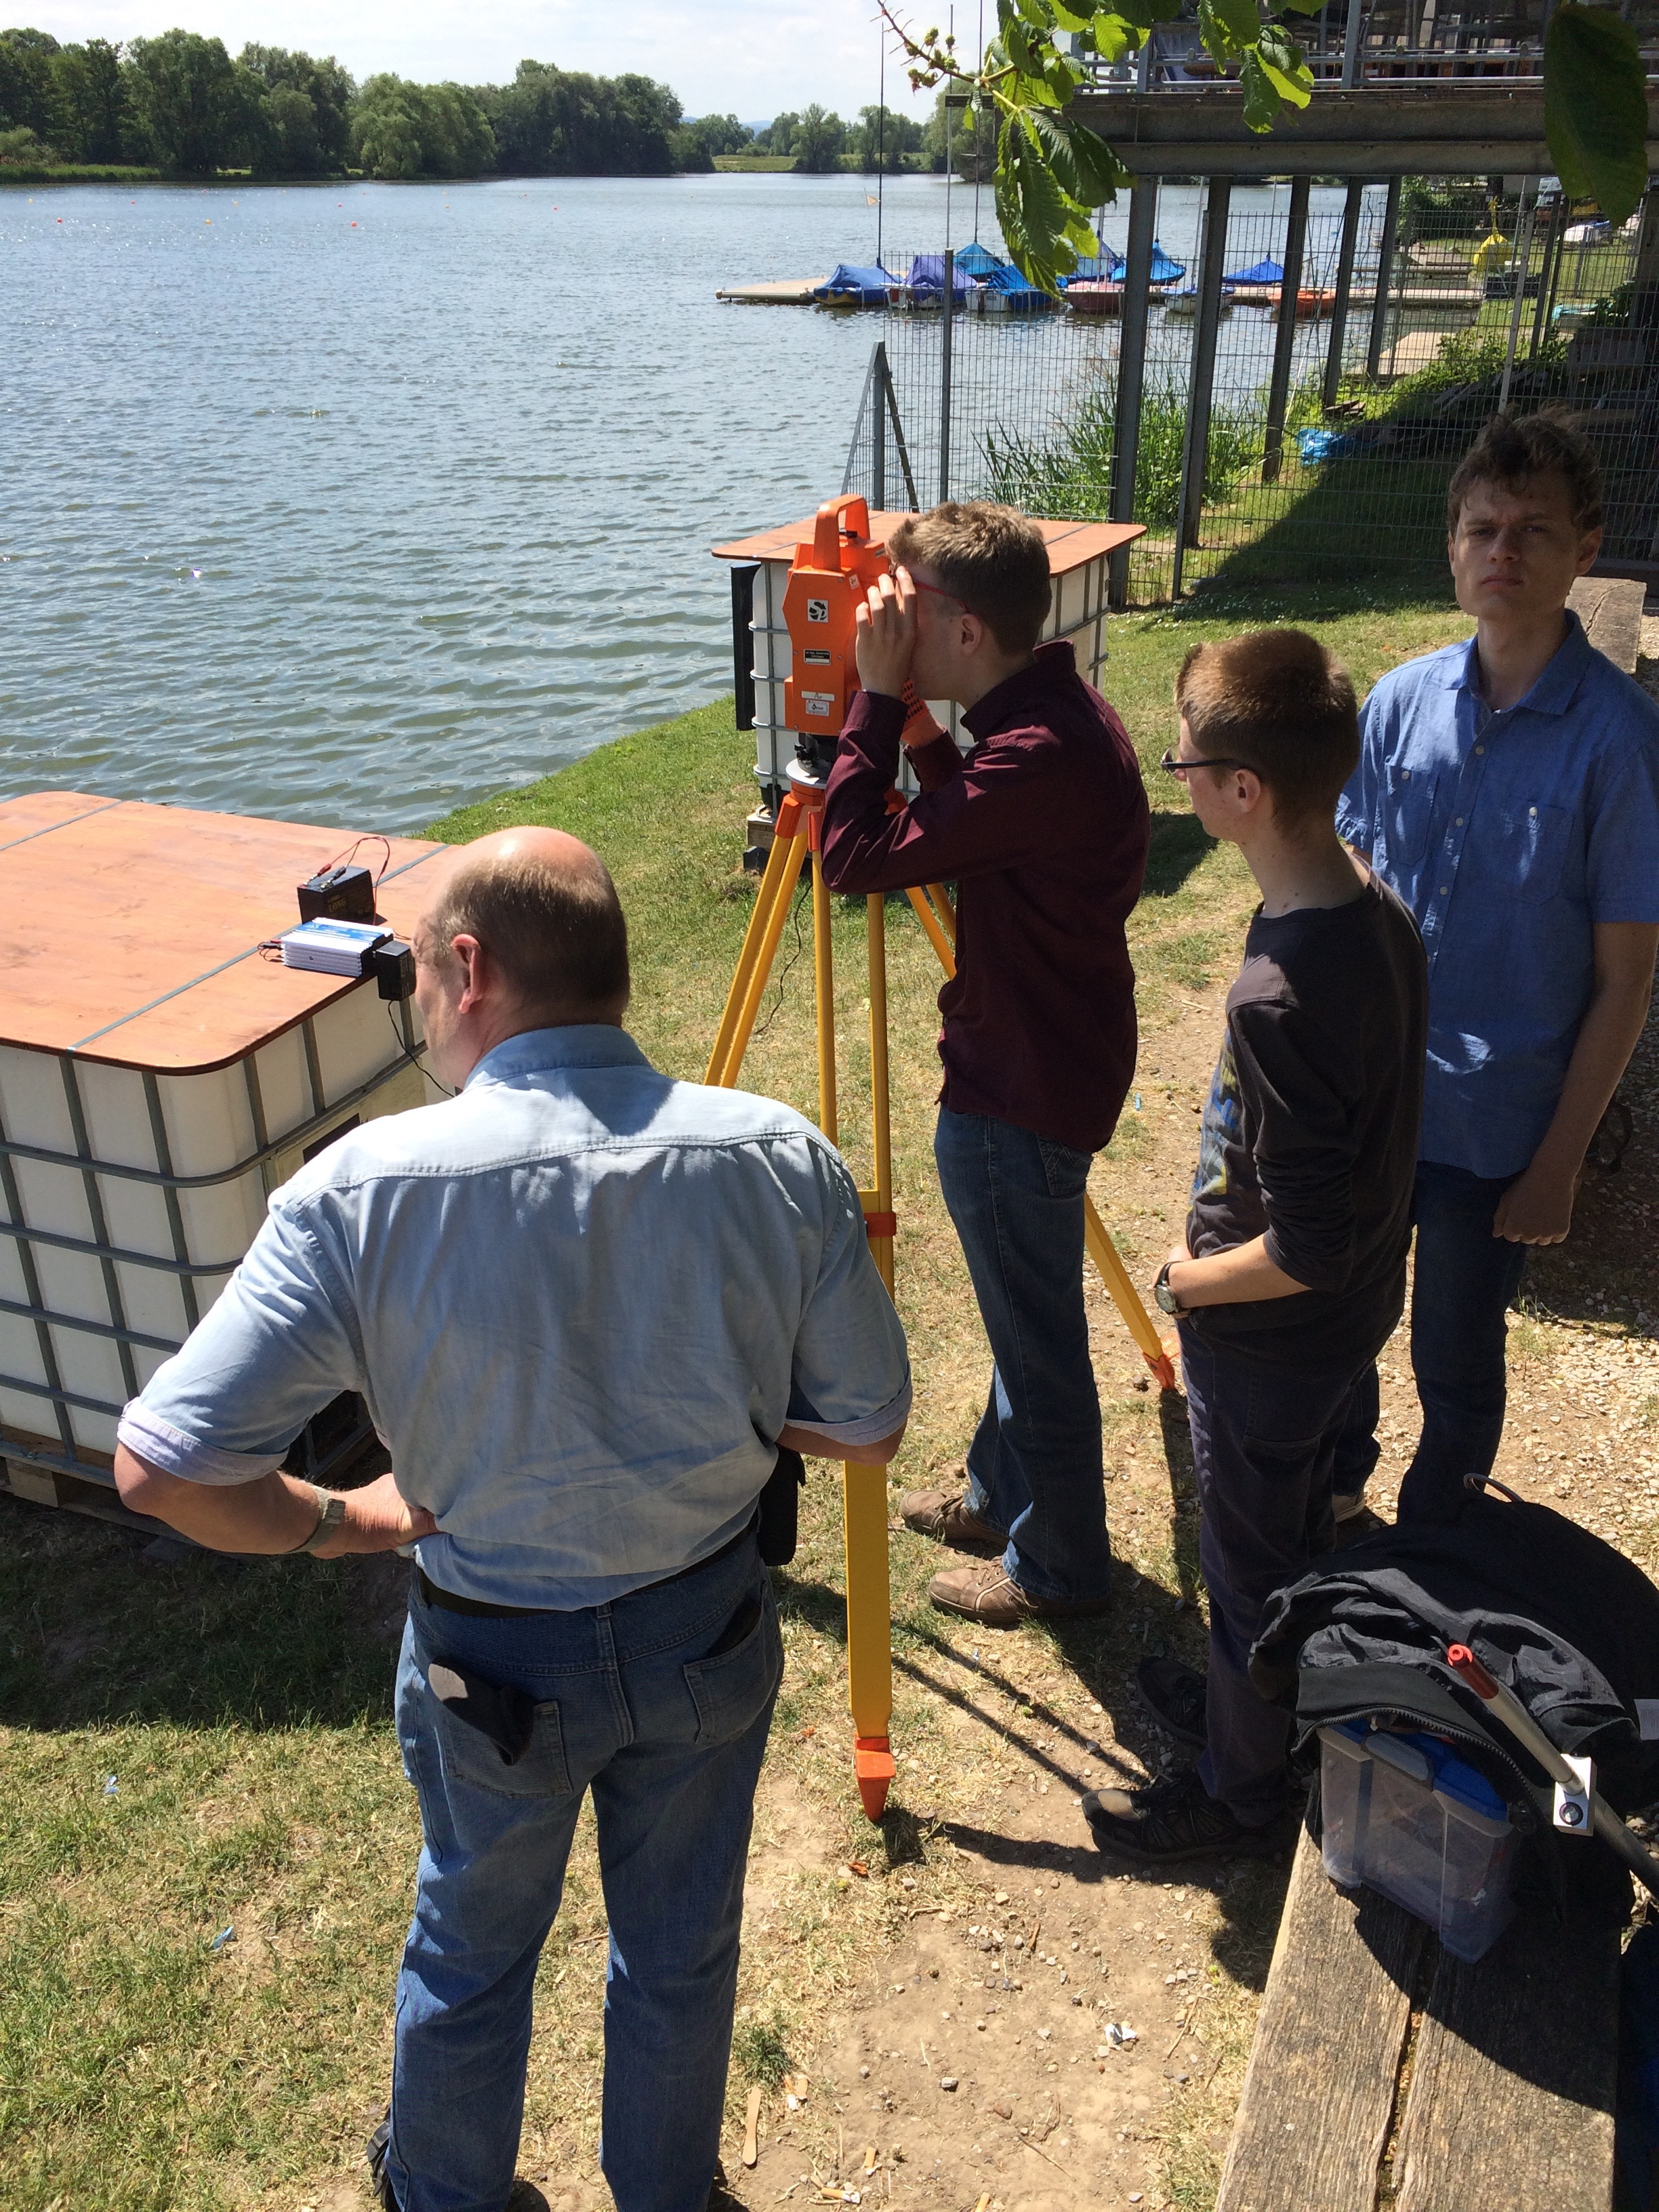
\includegraphics[height=10cm]{Fotos/Geodimeter}
	\caption{Kevin beim einstellen des Geodimeters.}
	\label{fig:geodimeter}
\end{figure}


\subsection{Temperatur}
Die Temperatur haben wir mit einem Pt1000-Widerstand vermessen.
Der Name verrät, dass der Messfühler aus Platin ist und bei $0\si{\celsius}$ einen Widerstand von $R_0=1000\si{\ohm}$ hat.
Der Widerstand hängt so von der Temperatur $\vartheta>0\si{\celsius}$ ab:
\begin{align}
	R(\vartheta)&=R_0\cdot\left(1 + A\vartheta + B\vartheta^2\right) \label{eq:Pt1000}
\end{align}
Die zugehörigen Konstanten findet man in Tabelle \ref{tab:Pt1000}.

\begin{table}[!htb]
	\centering
	\begin{tabular}{|c|c|}
		\hline
		R$_0$ & $1000 ~ \si{\ohm}$\\
		A   & $3.9083 \cdot 10^{-3} ~ \si{\celsius^{-1}}$\\
		B   & $-5.775 \cdot 10^{-7} ~ \si{\celsius^{-2}}$\\
		\hline
	\end{tabular}
	\caption{Kennwerte des Widerstandsthermometers}
	\label{tab:Pt1000}
\end{table}

Der Fehler der Temperaturmessung dieses Gerätes liegt bei
\begin{align}
	\Delta\vartheta=\pm (0.3~\si{\celsius}+0.005\vartheta)~.
	\label{eq:Pt1000_fehler}
\end{align}

Allerdings ist unser Sensor zwecks Wasserdichtigkeit mit einem dünnen Film Klebstoff beschichtet.
Dieser sollte nur die Reaktionszeit beeinflussen.
Das größere Hinderniss bei der Temperaturbestimmung lag bei uns am ADC (Analog-Digital-Converter), welcher die verstärkte Spannung in ein digitales Signal umwandelt.
Dessen Auflösung ist mit 16 Bit zwar schon recht gut, allerdings bedeutet dies, dass nur Spannungsunterschiede von xxxxxxxxxxxxxxxxxxxx V gemessen werden können, was einer Temperaturdifferenz von ca. xxxxxxxxxxxxxxxxxxxxxxxxxx$^\circ$ entspricht.


\subsection{Absorption}

\subsection{Echolot}
                                                                                                                                                                      
\section{Durchführung}
\label{sec:durchfuehrung}
Zur Messung eines Sees ist es notwendig, zunächst den Bereich, den man vermessen möchte sinnvoll einzuschränken und sich eine grobe Rasterung zu überlegen.
Dabei ist zu bedenken, dass für jeden Messpunkt ca. 3-5min eingerechnet werden müssen.
Auch müssen die Positionen, sofern sie mit dem Geodimeter ermittelt werden sollen, alle von einem Punkt am Ufer aus sichtbar sein.
Man könnte zwar das Geodimeter umstellen, jedoch würde dies zu einer enorm vergrößerten Unsicherheit des Ortes führen.

Die eigentliche Messung besteht darin, dass der Ruderer an einer Stelle anhält und den Messstab für das Geodimeter hochhält.
Gleichzeitig drückt die andere Person auf dem Boot den Knopf "`Start"' und lässt die Sonde langsam herunter.
Ist die Sonde auf dem Grund des Sees angekommen, so kann sie wieder hochgezogen werden.
Dies muss nicht so langsam geschehen, da sich bei Kontakt mit dem Boden teilweise Schlamm um die Sensoren legt, welche die Messung verfälschen.
Dieser muss gegebenenfalls nach Beendigung der Messung abgespühlt werden.


\subsection{Smartohone-App}
\label{sec:app}
Da bei der ersten Messung schon das Abfahren des relativ kleinen Göttinger Kiessees in einem Raster nicht leicht war, haben wir eine App für das Smartphone erstellt.
Mit das GPS-Modul des Smartphones liefert die aktuelle Position und stellt sie auf einer Karte dar.
Nun gibt es zwei Möglichkeiten:
\begin{itemize}
	\item Multi-Messung: Die Position wird ständig getrackt.
		Sobald sie sich verändert, wird diese in eine Datei geschrieben.
	\item Einzelmessung: Dies kann parallel zu der Multi-Messung passieren.
		Hierbei wird nur auf Knopfdruck auf den Button "`Einzelmessung"' ein einzelner Ort in eine andere Datei geschrieben.
		Außerdem wird die Position auf der Karte mit einer Stecknadel markiert und um die Position wird ein Radius eigezeichnet, der sich über einen Schieberegler einstellen lässt.
		Dies hat den Vorteil, dass man variabel die Rasterung anpassen kann.
\end{itemize}

Die App zeigt (wie in Abb. \ref{fig:appDetail} zu sehen) auch die Anzahl der aufgenommenen Datenpunkte an und die beiden Dateien, welche bei den Messungen angelegt werden.

Wurde die Messung an einem Ort nun beendet, kann man einfach so lange in eine Richtung fahren, bis man den roten Kreis um den letzten Datenpunkt erreicht hat.
Im Verlauf der Messung wird nun der ganze See systematisch mit den Kreisen überdeckt.

Am Ende des Messtages kann mit dem Knopf "`Senden"' nun eine Tabelle (s. Abb. \ref{fig:appTabelle}) geöffnet werden, welche die vorhandenen Dateien anzeigt.
Tippt man nun auf eine der Zeilen, so wird eine Mail erstellt, die schon voreingestellt die Mailadressen, Betreff und Inhalt, sowie die angehängte Datei besitzt.
Diese kann nun bequem mit einem Tippen versandt werden.


\begin{figure}[h]
  \centering
  \subfigure[Einzelne Datenpunkte an einer Stelle des Sees.\label{fig:appDetail}]
  {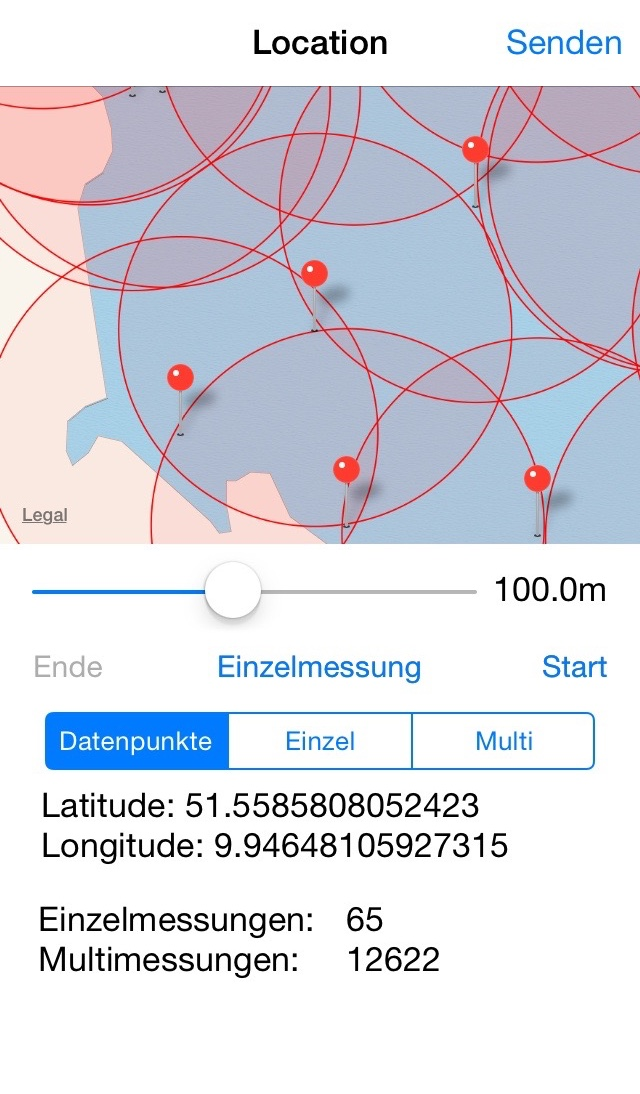
\includegraphics[width=0.32\textwidth]{Fotos/AppSeeDetail}}
  \hfill
  \subfigure[Übersicht über alle aufgenommenen Messpunkte in der App.\label{fig:appGesamt}]
  {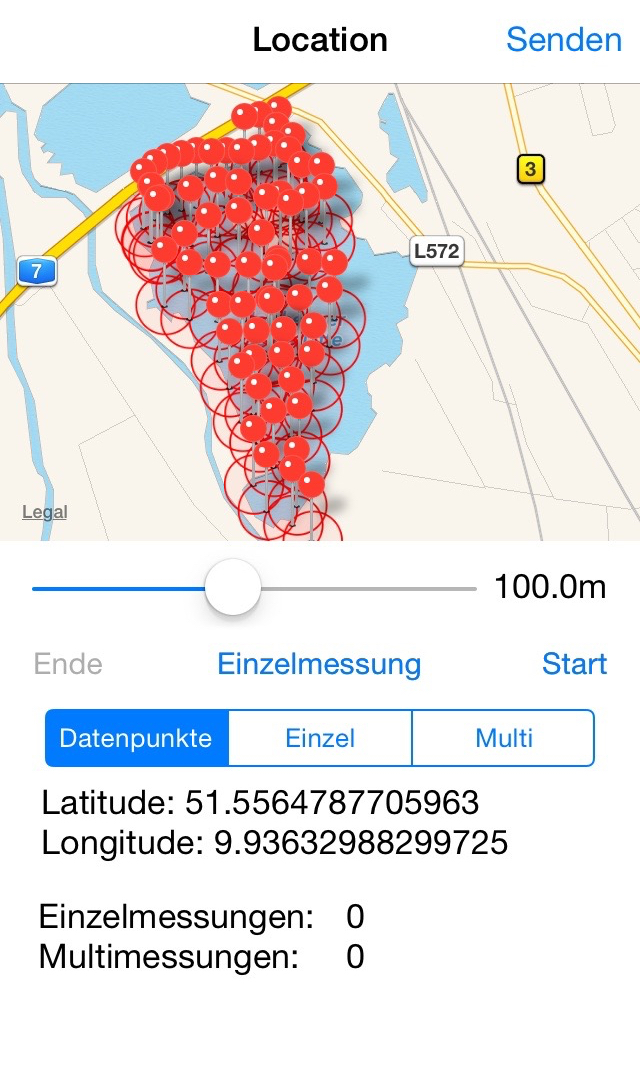
\includegraphics[width=0.32\textwidth]{Fotos/AppSeeKomplett}}
  \hfill
  \subfigure[Auswahl der zu versendenden Datei.\label{fig:appTabelle}]
  {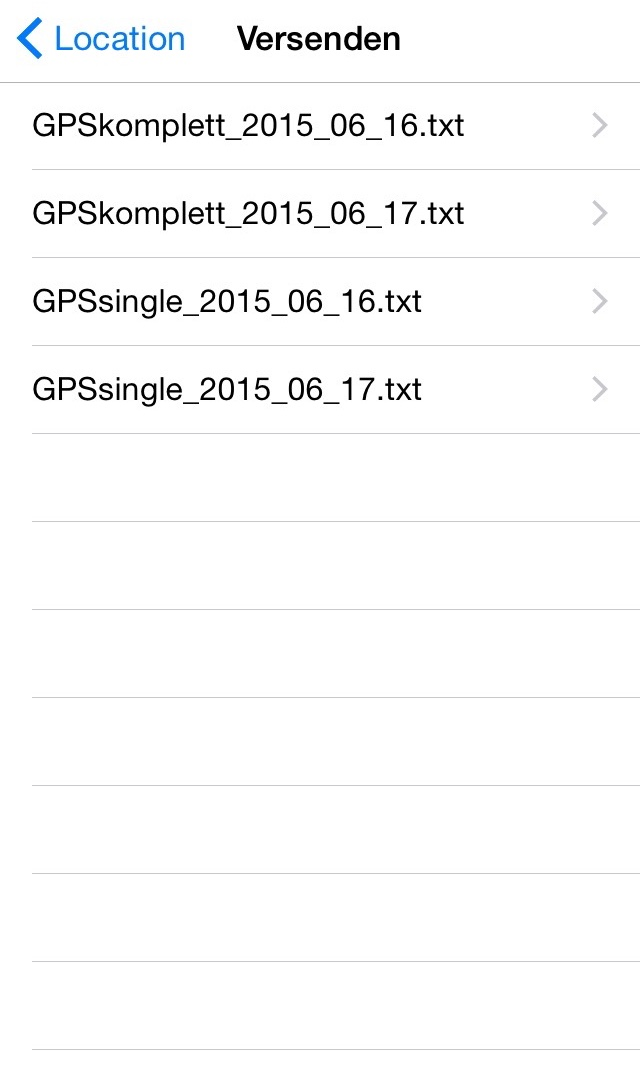
\includegraphics[width=0.32\textwidth]{Fotos/AppVersenden}}
  \caption{Screenshots der App.}
  \label{fig:appScreenshots}
\end{figure}

\section{Auswertung}
\label{sec:auswertung}

\subsection{Ortsbestimmung}

Unsere Befürchtung, dass das GPS-Signal zu ungenau ist, stellte sich als ungenau heraus.
Wir nutzten bei der zweiten Messung gleichzeitig einen GPS-Logger und die selbstgeschriebene Handy-App.
Durch Vergleich der beiden Messdaten erkennt man, dass sie sehr gut miteinander übereinstimmen.
Dies ist vielleicht auch zu erwarten, da beide ähnliche Signale bekamen.

Der GPS-Logger zeigte die Genauigkeit auf dem Display an, welche fast immer 3m betrug.
Diese hohe Genauigkeit, welche sich unter "`Normalbedingungen"' nur selten erreichen lässt, wird dadurch erklärt, dass wir auf einer weiten Fläche ohne große Hindernisse waren.
Somit gab es nichts, was die Signale der Satelliten reflektieren oder blockieren konnte.




\section{Diskussion}
\label{sec:diskussion}
\subsection{Druck}


\subsection{Echolot}


\subsection{Ortsbestimmung}


\subsection{Temperatur}
Bei der zweiten Messung zeigte sich in den Daten, dass die Werte der Temperatur augenscheinlich gleichzeitig drei Werte annehmen.
Bei genauerer Betrachtung der Messwerte fällt jedoch auf, wie in Abb. \ref{fig:tempSprung} zu erkennen, dass jeweils ungefähr 10 Messwerte auf einem niedrigen, dann auf einem mittleren, erneut auf einem niedrigen und dann wieder auf einem hohen Niveau liegen.
Dies  entspricht genau der Frequenz, mit der wir die LEDs angeschaltet haben (keine LED, blaue LED, keine LED, IR-LED).
Für beide Messungen benutzten wir den Micro-Controller als Stromquelle.
Dieser ist für Ströme von bis zu 350mA ausgelegt.
Augenscheinlich haben da die 50mA, welche die LEDs benötigten, die Stromzufuhr des ADCs so stark beeinflusst, dass die aufgenommenen Messwerte Temperatursprünge von biszu $4^\circ $C aufweisen.

\begin{figure}[h]
	\centering
	% GNUPLOT: LaTeX picture with Postscript
\begingroup
  \makeatletter
  \providecommand\color[2][]{%
    \GenericError{(gnuplot) \space\space\space\@spaces}{%
      Package color not loaded in conjunction with
      terminal option `colourtext'%
    }{See the gnuplot documentation for explanation.%
    }{Either use 'blacktext' in gnuplot or load the package
      color.sty in LaTeX.}%
    \renewcommand\color[2][]{}%
  }%
  \providecommand\includegraphics[2][]{%
    \GenericError{(gnuplot) \space\space\space\@spaces}{%
      Package graphicx or graphics not loaded%
    }{See the gnuplot documentation for explanation.%
    }{The gnuplot epslatex terminal needs graphicx.sty or graphics.sty.}%
    \renewcommand\includegraphics[2][]{}%
  }%
  \providecommand\rotatebox[2]{#2}%
  \@ifundefined{ifGPcolor}{%
    \newif\ifGPcolor
    \GPcolorfalse
  }{}%
  \@ifundefined{ifGPblacktext}{%
    \newif\ifGPblacktext
    \GPblacktexttrue
  }{}%
  % define a \g@addto@macro without @ in the name:
  \let\gplgaddtomacro\g@addto@macro
  % define empty templates for all commands taking text:
  \gdef\gplbacktext{}%
  \gdef\gplfronttext{}%
  \makeatother
  \ifGPblacktext
    % no textcolor at all
    \def\colorrgb#1{}%
    \def\colorgray#1{}%
  \else
    % gray or color?
    \ifGPcolor
      \def\colorrgb#1{\color[rgb]{#1}}%
      \def\colorgray#1{\color[gray]{#1}}%
      \expandafter\def\csname LTw\endcsname{\color{white}}%
      \expandafter\def\csname LTb\endcsname{\color{black}}%
      \expandafter\def\csname LTa\endcsname{\color{black}}%
      \expandafter\def\csname LT0\endcsname{\color[rgb]{1,0,0}}%
      \expandafter\def\csname LT1\endcsname{\color[rgb]{0,1,0}}%
      \expandafter\def\csname LT2\endcsname{\color[rgb]{0,0,1}}%
      \expandafter\def\csname LT3\endcsname{\color[rgb]{1,0,1}}%
      \expandafter\def\csname LT4\endcsname{\color[rgb]{0,1,1}}%
      \expandafter\def\csname LT5\endcsname{\color[rgb]{1,1,0}}%
      \expandafter\def\csname LT6\endcsname{\color[rgb]{0,0,0}}%
      \expandafter\def\csname LT7\endcsname{\color[rgb]{1,0.3,0}}%
      \expandafter\def\csname LT8\endcsname{\color[rgb]{0.5,0.5,0.5}}%
    \else
      % gray
      \def\colorrgb#1{\color{black}}%
      \def\colorgray#1{\color[gray]{#1}}%
      \expandafter\def\csname LTw\endcsname{\color{white}}%
      \expandafter\def\csname LTb\endcsname{\color{black}}%
      \expandafter\def\csname LTa\endcsname{\color{black}}%
      \expandafter\def\csname LT0\endcsname{\color{black}}%
      \expandafter\def\csname LT1\endcsname{\color{black}}%
      \expandafter\def\csname LT2\endcsname{\color{black}}%
      \expandafter\def\csname LT3\endcsname{\color{black}}%
      \expandafter\def\csname LT4\endcsname{\color{black}}%
      \expandafter\def\csname LT5\endcsname{\color{black}}%
      \expandafter\def\csname LT6\endcsname{\color{black}}%
      \expandafter\def\csname LT7\endcsname{\color{black}}%
      \expandafter\def\csname LT8\endcsname{\color{black}}%
    \fi
  \fi
    \setlength{\unitlength}{0.0500bp}%
    \ifx\gptboxheight\undefined%
      \newlength{\gptboxheight}%
      \newlength{\gptboxwidth}%
      \newsavebox{\gptboxtext}%
    \fi%
    \setlength{\fboxrule}{0.5pt}%
    \setlength{\fboxsep}{1pt}%
\begin{picture}(7200.00,5040.00)%
    \gplgaddtomacro\gplbacktext{%
      \csname LTb\endcsname%
      \put(682,1126){\makebox(0,0)[r]{\strut{}$18$}}%
      \put(682,1886){\makebox(0,0)[r]{\strut{}$19$}}%
      \put(682,2647){\makebox(0,0)[r]{\strut{}$20$}}%
      \put(682,3407){\makebox(0,0)[r]{\strut{}$21$}}%
      \put(682,4168){\makebox(0,0)[r]{\strut{}$22$}}%
      \put(1738,484){\makebox(0,0){\strut{}$3300$}}%
      \put(2925,484){\makebox(0,0){\strut{}$3320$}}%
      \put(4112,484){\makebox(0,0){\strut{}$3340$}}%
      \put(5300,484){\makebox(0,0){\strut{}$3360$}}%
      \put(6487,484){\makebox(0,0){\strut{}$3380$}}%
    }%
    \gplgaddtomacro\gplfronttext{%
      \csname LTb\endcsname%
      \put(176,2739){\rotatebox{-270}{\makebox(0,0){\strut{}$^\circ$ C}}}%
      \put(3808,154){\makebox(0,0){\strut{}Messpunkt}}%
      \csname LTb\endcsname%
      \put(5816,4602){\makebox(0,0)[r]{\strut{}Temperatur}}%
    }%
    \gplbacktext
    \put(0,0){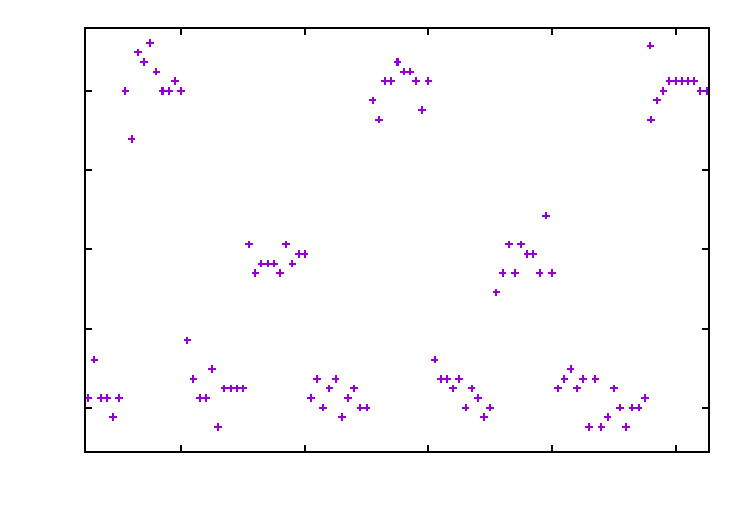
\includegraphics{tempSprung}}%
    \gplfronttext
  \end{picture}%
\endgroup

	\caption{Vergrößerte Darstellung einer Temperaturkurve.}
	\label{fig:tempSprung}
\end{figure}



\subsection{Absorption}



\subsection{Messprobleme und verworfene Ideen}
Unsere erste Idee war die, ein ferngesteuertes U-Boot zu bauen, was die Sensoren an Bord hat.
Dies stellte sich jedoch sehr schnell als nicht durchführbar heraus, da es keine geeigneten Modellbauten gab und da die komplette Technik mit Stromversorgung unter Wasser luftdicht sein müsste.
Daher kamen wir auf die Idee, eine ferngesteuerte Plattform zu bauen, welche die Sonden mit einer Winde ferngesteuert herunterlässt.
Dies verwarfen wir jedoch auch sehr schnell, da die Fernsteuertechnik einen großen Teil unserer Arbeit ausgemacht hätte, was wissenschaftlich wenig interessant ist.
Auch hätten wir Probleme bekommen, falls sich zum Beispiel die Sensoren in Wasserpflanzen verfangen.

So entschieden wir uns für die simplere Umsetzung, ein Ruderboot zu nehmen und die Stromversorgung, sowie die Datenverarbeitung im Boot zu betreiben und nur die Sensoren an den Kabeln herunter zu lassen.


Wir hatten zunächst noch vor, weitere Sensoren zu verwenden:
\begin{itemize}
	\item \textit{el. Leitfähigkeit}: Funktionierte nicht, da wir dafür Wechselspannungen mit mindestens 50V benötigt hätten.
		Dies wäre notwendig, da sich sonst an den Elektroden durch Eletrolyse Salze angelagert hätten, welche für eine höhere gemessene Leitfähigkeit gesorgt hätten.
		Die Leitfähigkeit alleine ist kein Maß für den Salzgehalt, der auch noch von anderen Größen maßgeblich beeinflusst wird.
		So konnten wir den Sensor, welchen Jan bereits besorgt hatte, nicht einsetzen.
	\item \textit{pH-Wert}: Der pH-Wert wäre auch eine interessante Messgröße gewesen.
		Allerdings wäre zur Kallibration mindestens eine Pufferlösung notwendig gewesen.
		Ausschlaggebend war, dass wir zu den preislich akzeptablen Sensoren keine vernünftigen Datenkurven finden konnten, da diese augenscheinlich nur für fertige Geräte ausgelegt sind.
\end{itemize}


\bibliography{literatur}
\bibliographystyle{babalpha}
\end{document}
